\chapter{Déroulement du Stage}
\label{main}

Cette section va présenter les différentes tâches accomplies au cours de la période de stage.
Celles-ci ne sont globalement pas présentées dans un ordre chronologique, elles sont simplement regoupées par thèmes.

% -=+=-
% RESUME
% -=+=-

\section{Information sur le sujet}

Pour pouvoir débuter le stage correctement, il était nécessaire de s'informer correctement sur le sujet traité et les sujets adjascents.
Il était aussi important de pouvoir se familiariser avec les usages des publication scientifique, de pouvoir s'entraîner a correctement
lire ce genre de publications.
C'est pourquoi on m'as proposer plusieurs articles à décortiquer, que j'ai résumé simplement, tout au long du stage.

\subsection{Format et Rendu}

Le format de résumé que j'ai choisi est ASCIIDOC, qui permet un formattage similaire à Markdown (avec un peu plus de possibilités), et une exportation facile en HTLM grâce à \href{https://asciidoctor.org/}{asciidoctor}.

Les sources de ces documents sont hébergées sur un dépot mise à ma disposition sur le groupe GitHub du groupe PROGRESS:
\url{https://github.com/labri-progress/llm-study-zoo}

L'affichage Github n'éttant pas complet (n'affiche pas les documents importés et les formules mathématiques, entre autres), j'ai décidé de rendre disponible un version rendue sur ma page CREMI:
\url{https://maxime-pico.emi.u-bordeaux.fr/stage-labri/llm-study-zoo/}.


\subsection{Résumés}

Cette section passera rapidement sur les différents sujets présentés dans les articles que l'on m'a confié, ainsi que ce qui a pu etre tiré de l'article pour etre employé au cours du stage.
Pour des résumés plus détaillés, il est préférable d'aller voir \href{https://maxime-pico.emi.u-bordeaux.fr/stage-labri/llm-study-zoo/}{le rendu html sur ma page CREMI}


\subsubsection{Empirical study on Code Completion Tools \cite{evalcodecompquality}}

Cet article présente une expérience de comparaison de performances entre
3 modèles de complétions sur un dataset de petites fonction avec leurs documentation.

Ce type d'experience m'as permi de voir le type d'expérimentation possible pour ce genre d'outils ainsi que
les types de mesures qui puissent être utilisées.


\subsubsection{Offline evaluation of Code Completion Tools \cite{llm-online-offline}}

Cet article présente une expérience de comparaison de performances entre
3 modèles de complétions, cette fois-ci open-sources, sur \href{https://github.com/VHellendoorn/Code-LMs#datasets}{un dataset multilangues} \cite{dataset-code-lm}.

Comme le précendent, il s'agit ici de voir la mise en place de l'expérience et les différents types de mesures.


\subsubsection{Online evaluation of Code Completion Tools \cite{llm-online-offline}}

Cette section fait partie de l'article précendant, il s'agit de la deuxième partie de l'expérience.
Il s'agit ici d'évaluer d'un point de vue qualitatif et quantitatif les différents modèles "dans la nature",
c'est à dire directement en les testant auprès de développeurs pendant leurs sessions de travail.

On est ici sur un expérience plus proche que ce qui peut nous interesser pour notre sujet: une expérimentation directement avec des développeurs.


\subsubsection{Grounded Copilot: How Programmers Interact with Code-Generating Models \cite{grouded}}

Cette publication m'as été proposée car c'est une "grounded theory".
Ce type de publication cherche à faire emmerger des hypothèses à partir de données récolté sur une expérience.

Ici les chercheurs on mis en avant différents modes d'intéraction vis-à-vis des outils de suggestion comme GitHub Copilot (mode \emph{acceleration} et mode \emph{exploration}).
Il pourrait-être interressant de les faire resortir dans nos expérience, et d'integrer cette différenciation de phases dans l'analyse des données.


\subsubsection{CodeAid: A classroom deployment of an LLM-based programming assistant \cite{codeaid}}

Il s'agit ici d'une expérience mise en place sur une classe universitaire durant un semestre visant a observer les comportement des étudiants
face à un outils d'assistance à la programmation.
Cet article est très intéressant, il nous permet de voir le type d'expériences qui peut etre mener pour notre projet, ce qu'il est possible de mettre en place.

Dans cette expérience, les chercheurs on créé une extensions pour éditeur avec une interface ayant plusieurs modes d'interactions.
L'idée était de voir ce que les étudiants allaient utiliser, et dans quel contexte.


\subsubsection{Productivity Assessment of Neural Code Completion \cite{productivity-assess}}

Cet article est l'un des dernier que j'ai traité, le résumé n'est pas complet, cependant, il nous a renseigné sur la manière dont on peut
quantifier la productivité (ressentie) grâce au taux d'acceptation des complétions proposées par les extensions.

% -=+=-
% EXPLO
% -=+=-

\section{Exploration des outils a tester}
\label{explo}

Il existe de nombreux outils permettant la suggestion de code via des modèles prédictifs, il s'agit donc de trouver celui qui va convenir le mieux au type d'expériences que l'ont veut mener.

On a vu dans la séquence précedante quelques article qui utilisait justement ce genre d'outils, mais avec des approches différentes:

\begin{itemize}
  \item \textbf{En utilisant un model/une extension pré-éxistante} et en observant les comportements \cite{grouded}, ou en outillant l'IDE \cite{productivity-assess}.
  \item \textbf{En créant un outil autour d'un model distant} tel que CodeAID \cite{codeaid}, qui discute via des API pour suggerer completions, ou d'autre proxy comme \href{https://continue.dev}{continue.dev}.
  \item \textbf{En hébergeant soit-même un modèle}, soit sur un serveur \cite{llm-online-offline}, soit sur la machine du développeur.
\end{itemize}

Pour des contrainte de temps et de complexité de mise en place, nous somme résté sur la première option et avont utilisé GitHub Copilot, auquel j'ai accès gratuitement de part mon statut d'étudiant \cite{gh-students}.
De plus, de nombreux autres outils nécessitaient beaucoup de performances à faire tourner, nottament pour les models locaux, ou ne fonctionnaient pas du tout.

% -=+=-
% CODEGRITS
% -=+=-

\newpage
\section{Prise en main et modification de CodeGRITS}

CodeGRITS est un outils d'enregistement pour des sessions de développement sous IntelliJ IDEA (et IDE dérivés), Il m'a été proposé par mes encadrant comme un
piste potentielle pour pouvoir enregister les intéractions avec les models/extensions de completion de code assités par IA.

Comme dit précedement dans \ref{explo}, le model/extension sur lequel mon stage s'est concentré est GitHub Copilot, c'est l'outils autour duquel j'ai intrumenté CodeGRITS.

Le but ici était de chercher si est possible d'utiliser CodeGRITS avec GitHub Copilot pour récuperer des informations pendant la session de développement, tel que la suggestion d'un complétion et l'acceptation.

Tout les changements apportés à l'extensions sont publiés sur un fork de la repo sur mon compte GitHub personel: \url{https://github.com/Syudagye/CodeGRITS}


\subsection{Exploration}

Dans un permier temps, il a fallu explorer l'extension, voir ce qui était proposé par l'outil et ainsi voir ce qui allait être nécessaire à ajouter
pour arriver a quelque chose qui nous convienne dans le contexte d'un potentielle experience.


\subsubsection{Mise à jour}

La première étape était de faire foncionner l'extension CodeGRITS.
Celle-ci étant faite pour les IDE IntelliJ antérieurs aux versions 2024 (voir figure \ref{codegrits-old-build-version}), il a fallu l'adapter
(c.f. commit \href{https://github.com/codegrits/CodeGRITS/commit/cdb10bcba529d050bfcb6c3693256f0e18450dad}{cdb10bc}).
En effet, afin d'eviter de chercher un moyens de downgrade mon installation d'intellij sur mon environement de travail (installé sous NixOS avec Flatpak),
j'ai préféré mettre à jour l'extension elle-même.
Même si celà aurais pû poser de potentiels problèmes de compatibilité, nottament avec l'api d'IntelliJ, ça aurait été quelque chose d'intéressant à faire, et a proposer aux développeurs
de l'extensions pour améliorer leur outil.


\subsubsection{Données}

L'extension récupère des données sur la session de développement et les engeristre dans un dossier à la racine du projet ouvert dans l'IDE.
Il a fallu donc décortiquer la structure de ce dossier et des fichiers qui y sont contenus. Heureusement, ces données sont faite pour être facilement exploitables, la structure du dossier est donc très explicite:

\begin{itemize}
  \item Un dossier \lstinline{archives} contenant des sauvegardes des fichiers sources modifiés
  \item Un dossier \lstinline{screen_recording} contenant un fichier video de l'écran pendant la session
  \item Un fichier \lstinline{ide_tracking.xml} contenant différents événements émanant de l'éditeur pendant la session
\end{itemize}

Ce qui nous intéresse là-dedans sont les données contenues dans les fichier xml, car c'est ici qu'il peut y avoir des évenements pertinants dans le contexte de Copilot.

Malheureusement, celà n'as pas été completement le cas: En effet, seul un événement relatif à l'insersion d'un complétion dans le texte source
(voir figure \ref{apply-inlay-action}) n'est enregisté.

\begin{figure}
  \centering
  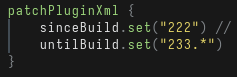
\includegraphics[width=7cm]{images/codegrits-wrong-version.png}
  \caption{Commande limittant les version utilisable d'IntelliJ}
  \label{codegrits-old-build-version}
\end{figure}

\begin{figure}
  \centering
  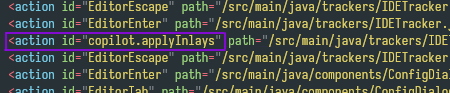
\includegraphics[width=10cm]{images/apply-inlay-action.png}
  \caption{Entrée du fichier \lstinline{ide_tracking.xml} référant à un évenement de complétion accéptée}
  \label{apply-inlay-action}
\end{figure}


\subsection{Modification}

Après avoir identifié les points manquants de l'extension CodeGRITS, il fallait maintenant trouver comment pallier à ce manque
en modifiant l'extension pour nos usages spécifiques.
À ce stade, il nous faut un moyens de tracker les moment ou l'extension Copilot viens suggerer du code au développeur, et que celui ci est visible
en grisé dans l'éditeur.

Plusieurs pistes on été envisagées, comme intercepter le traffic réseau entrant dans l'IDE, mais cela posait beaucoup de problème, nottament avec SSL pour décoder les paquets HTTPS.

Une approche beaucoup plus simple consistait à regarder les \emph{inlays} qui apparaissent dans l'éditeur,
c'est à dire les petits textes virtuels qui viennent donner des indications directement dans le viewport de l'éditeur de fichier,
comme par exemple le nom des paramêtre des fonctions, etc.
Ces \emph{inlays} sont gérés pour chaque fichier ouvert par un \emph{InlayModel}, auquel on peut attacher un listener afin de réagir
à la création / modification / destruction de ces inlays (voir Figure \ref{inlay-listener}).

Cependant, un fois cet accès acquit, il faut pouvoir récuperer les informations qui nous intéressent, ici le code proposé par GitHub Copilot.
Pour ce faire, il faut pouvoir détécter quel inlay nous intéresse, et récuperer les informations au bon endroit.

\begin{figure}
  \centering
  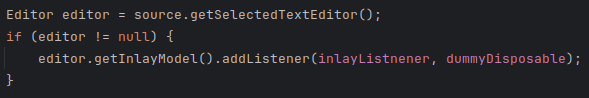
\includegraphics[width=10cm]{images/inlay-listener.png}
  \caption{Ajout d'un listener lors de l'ouverture d'un fichier}
  \label{inlay-listener}
\end{figure}


\subsubsection{Decompilation de Copilot}

GitHub Copilot n'étant pas du logiciel libre, il est impossible de regarder sont code de manière direct dur un depot publique, il faut donc trouver un autre moyens.
Heureusement, IntelliJ IDEA étant construit avec des technologies utilisant Java et la JVM, ses plugins aussi, il est donc possible de facilement décompiler l'extension afin de s'assurer de son fonctionnement.

Gâce à l'outil open source \emph{\href{https://java-decompiler.github.io/}{Java Decompiler}}, il est possible de retranscrir du bytecode executable par la JVM en code source java lisible (exemple Figure \ref{copilot-inlay-renderer}).
Sur l'image \ref{copilot-inlay-renderer}, on peut y voir une partie du code décompilé qui nous sera utile dans notre contexte: il s'agit du champ contenant le text qui s'affiche dans l'éditeur
quand Copilot veut nous suggerer quelque chose.

Comme on peut voir, il s'agit d'un champ privé, tout comme la classe qui l'abrite, mais java nous permet tout de même d'y acceder par des moyens détournés.

\begin{figure}
  \centering
  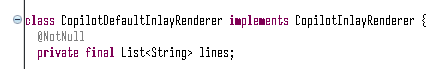
\includegraphics[width=10cm]{images/copilot-renderer-class.png}
  \caption{decompiled class of the inlay renderer in copilot's intellij plugin}
  \label{copilot-inlay-renderer}
\end{figure}


\subsubsection{Manipulation de la JVM}

Java est un language orienté objet, qui est compilé et éxécuté au sein d'une machine virtuelle, la JVM.
Les différentes visibilité des objets ne sont pas forcement garanties pendant l'execution du code comme elles le sont à la compilation.
Il est donc possible, en passant par des objets de la librairies standarde de Java, d'accèder à des champs privés de classes privés présentes
dans le contexte de la JVM courrante.

Dans l'adaptation de CodeGRITS que j'ai réalisé, je suis simplement allé chercher le champ \lstinline{lines} de l'objet renderer si il existait (voir \ref{getting-the-lines}).
Pour faire celà, Java propose dans la class \emph{Class<T>} un méthode permettant d'optenir un champ déclaré: \lstinline{getDeclaredField(String name)}.
Celle-ci nous permet d'intéragir avec le champ et de nottament modifier son accessibilité, et suite à quoi il est possible, peu importe la visibilité originale du champ,
d'acceder aux données qu'il renferme.

Ce procédé peut toutefois generer des exceptions d'accès illégal, d'où la présence d'un bloque \emph{try/catch} sur l'image \ref{getting-the-lines}.
Ettonement, pendant l'utilisation de cette modification, aucune de ces erreur ne m'as été renvoyée, il semblerai donc que cette methode fonctionne correctement.

\begin{figure}
  \centering
  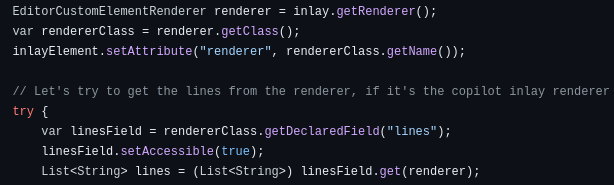
\includegraphics[width=15cm]{images/getting-the-lines.png}
  \caption{Récupération des données dans l'objet renderer de Copilot}
  \label{getting-the-lines}
\end{figure}

% -=+=-
% DATA
% -=+=-

\newpage
\section{Analyse des données}

Afin de pouvoir tirer profit des données produites par CodeGRITS, il a fallut chercher des outils permettant de lire et d'afficher les données produites.

Les données pertinantes pour nous sont celles des événements de GitHub Copilot, et ceux-ci sont présents dans le fichier ide\_tracking.xml.

\subsection{Parsing}

Dans un premier temps, je me suis intéressé au librairies de l'ecosystem Rust pour lire et afficher les données (nottement \emph{serde} et \emph{plotters}),
mais il s'avère que ce n'était vraiment pas pratique pour ce que l'on veut en faire.

Je me suis donc rabattu sur Python, qui possède un très solide arsenal pour l'analyse de données, nottament grâce aux fameuses librairies \emph{numpy} et \emph{pandas}.
De plus, la déserialisation des fichiers XML est déja incluse dans la libraries standarde du language, gâce à \href{https://docs.python.org/3/library/xml.etree.elementtree.html}{xml.etree.ElementTree},
ce qui le rends beaucoup plus pratique.
Ce module permet aussi d'acceder aux elements du document xml en utilisant la notation xpath.

\subsection{Plotting}

Pour l'affichage des donées, nous nous somme donner l'objectif de les présenter sous la forme d'une timeline, avec des événements de GitHub Copilot (propositions et acceptations).

La première approche à été de simplement le présenter avec \emph{matplotlib}, un module python très utilisé dans la communauté scientifique.
Malheureusement, les graphs qui en résultent sont seulement des images, et ne sont donc pas intéractifs et difficilement lisible, comme on peut le constater sur l'image \ref{matplotlib-timeline},
qui est un morceau d'un graph résultant d'une session de développement test.

Pour pouvoir acceder a plus d'interactibilité, on m'as donc orienté vers des librairies javascript tel que \href{https://d3js.org}{d3js}.
Malheureusement, beaucoup ne proposent pas de module permettant de generer des timeline comme nous voulions, et les quelques depot git qui semblaient pouvoir nous aider étaient abandonés depuis longtemps
et ne semblaient pas etre facilement utilisable (dépendant de version trop anciennes).

Malgrès ça, j'ai finalement trouvé \href{https://plotly.com/python/}{plotly} qui permet de créer exactement le type de timeline dont nous avont besoin (voir image \ref{cool-plot}),
c'est à dire un visuel où tout les événements on leur couleur propre, que l'on puisse zoomer et regarder des détails pour chaque événement en cliquant dessus.
Vous trouverez un rendu également sur ma page CREMI à l'adresse suivante: \url{https://maxime-pico.emi.u-bordeaux.fr/stage-labri/llm-study-zoo/timeline.html}
C'est un bon début ici, mais il serait bien plus intéressant de pouvoir pousser la visualisation plus loin, afin d'avoir une vue d'ensemble plus facile à comprendre au premier coup d'oeuil
(voir les travaux de Roberto Milleni \cite{cool-plot} et l'image \ref{ref-timeline}).

\begin{figure}
  \centering
  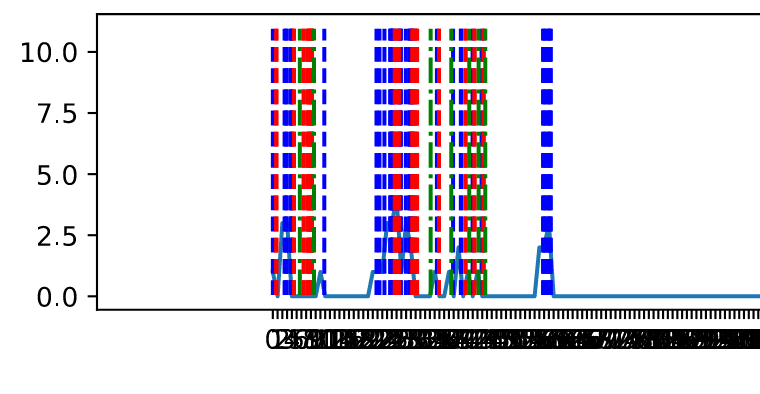
\includegraphics[width=15cm]{images/matplotlib-timeline.png}
  \caption{Première visualisation d'une session avec matplotlib}
  \label{matplotlib-timeline}
\end{figure}

\begin{figure}
  \centering
  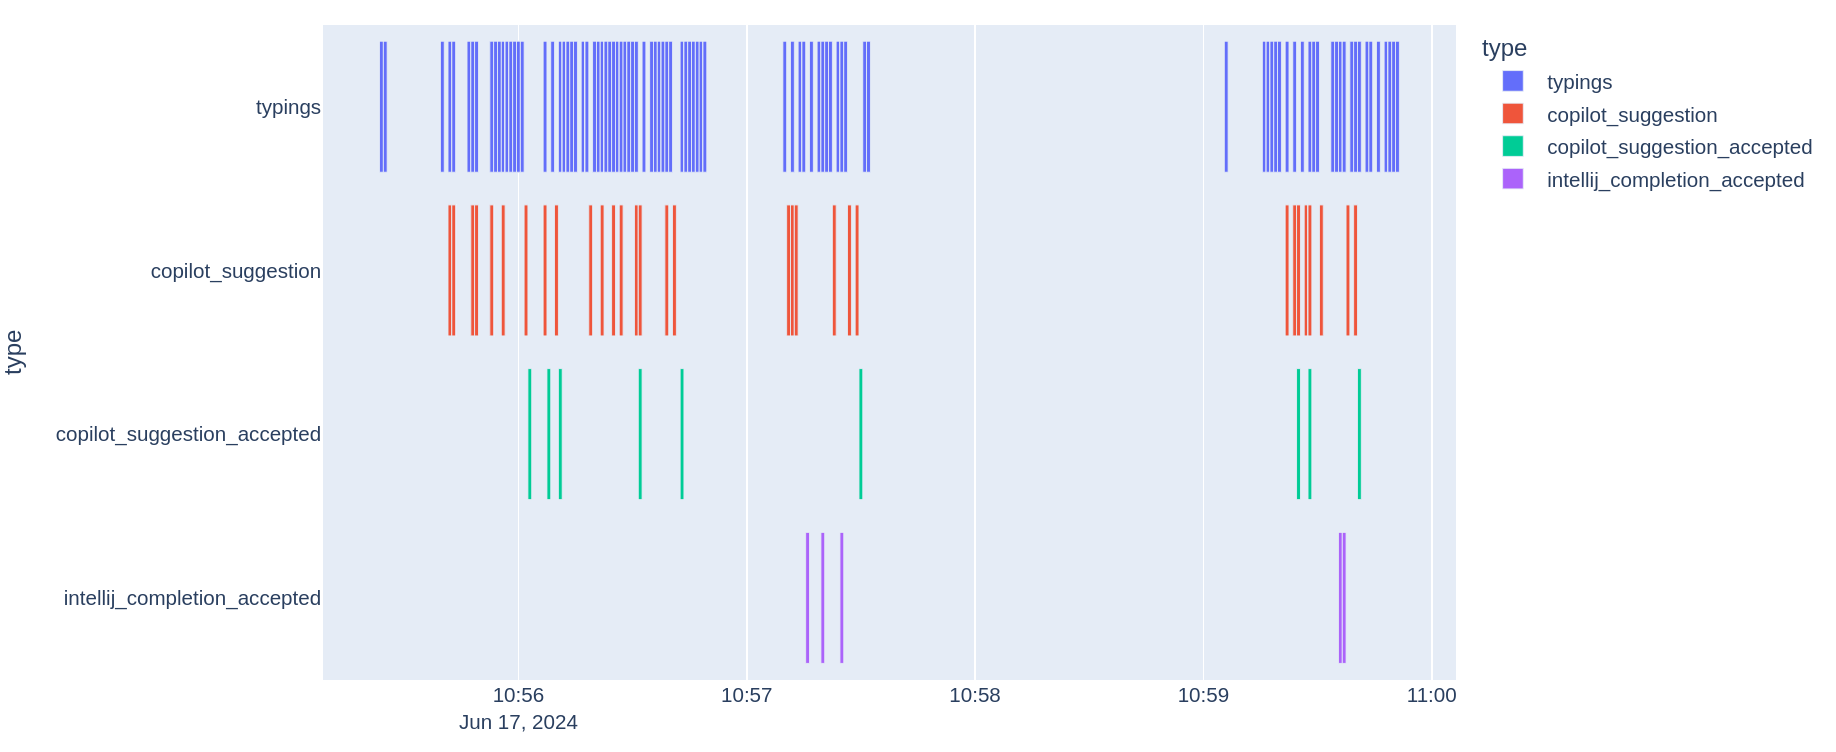
\includegraphics[width=15cm]{images/cool-plot.png}
  \caption{Aperçu de la visualisation plotly}
  \label{cool-plot}
\end{figure}

\begin{figure}
  \centering
  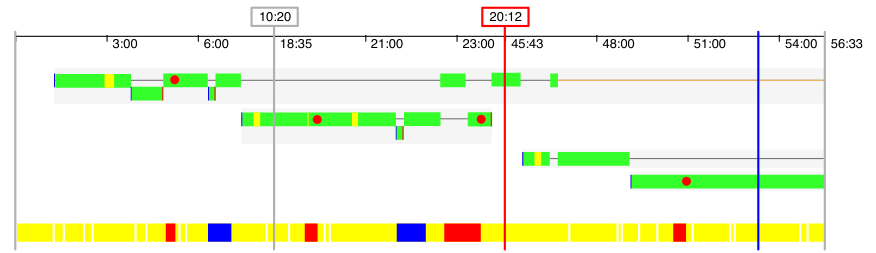
\includegraphics[width=15cm]{images/ref-timeline.png}
  \caption{Inspiration du model de timeline \cite{cool-plot}}
  \label{ref-timeline}
\end{figure}

% -=+=-
% THESIS
% -=+=-

\newpage
\section{Soutenances de thèses (bonus)}

Vers la fin du mois de juin, j'ai pu assister a deux soutenances de thèses au sein du LaBRI.
Celle de Christophe CASSEAU \cite{these-casseau}, et celle de Corentin LATAPPY \cite{these-latappy}.
Ce fut une expérience très enrichissante et motivante pour moi, et m'ont conforté dans l'idée d'aller vers ce chemin d'études.
Cela sort un peu du contexte du stage, mais il s'agit toujours pour moi de voir comment fonctionne le milieu de la recherche, et ce fut donc de très bonnes opportunités de s'y plonger.
